\documentclass[../Head/Main.tex]{subfiles}
\begin{document}
	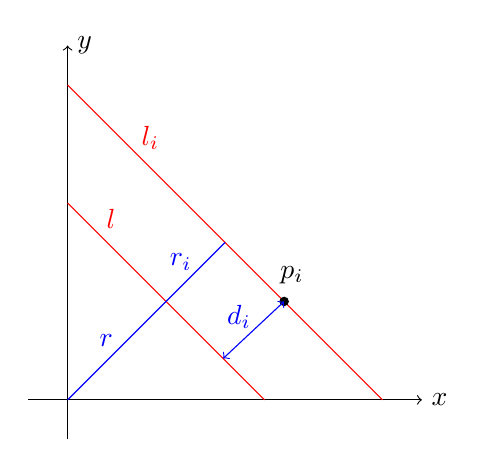
\begin{tikzpicture}
		\draw [->](0,-0.5)--(0,4.5) node[right]{$y$};
		\draw [->](-0.5,0)--(4.5,0) node[right]{$x$};
		\draw [red] (2.5,0) -- (0,2.5); 
		\draw [red] (4,0) -- (0,4); 
		\draw [red] (0.55,2.05) node[above]{$l$};
		\draw [red] (1.05,3.05) node[above]{$l_i$};
		\draw [blue] (0,0) -- (2,2);
		\draw [blue] (0.70,0.75) node[left]{$r$}; 
		\draw [blue] (1.70,1.75) node[left]{$r_i$};
		\filldraw (2.75,1.25) circle (1.5pt);
		\draw (2.85,1.35) node[above]{$p_i$};
		\draw [<->, blue] (1.975,0.525) -- (2.75, 1.25);
		\draw [blue] (2.45,1.05) node[left]{$d_i$};
	\end{tikzpicture}
\end{document}